\documentclass[oneside]{book}
\usepackage[utf8]{inputenc}
\usepackage{amsmath}
\usepackage{amssymb}
\usepackage{amsfonts}
\usepackage{tikz,pgfplots}
\usepackage{geometry}
\geometry{
  bottom=15mm
}
\usepackage{textcomp, gensymb}
\usepackage{hyperref}
\hypersetup{
    colorlinks=true,
    linkcolor=blue,
    filecolor=magenta,      
    urlcolor=cyan,
    }
\usepackage{background}
\backgroundsetup{
scale=1,
color=black,
opacity=0.5,
angle=0,
contents={%
  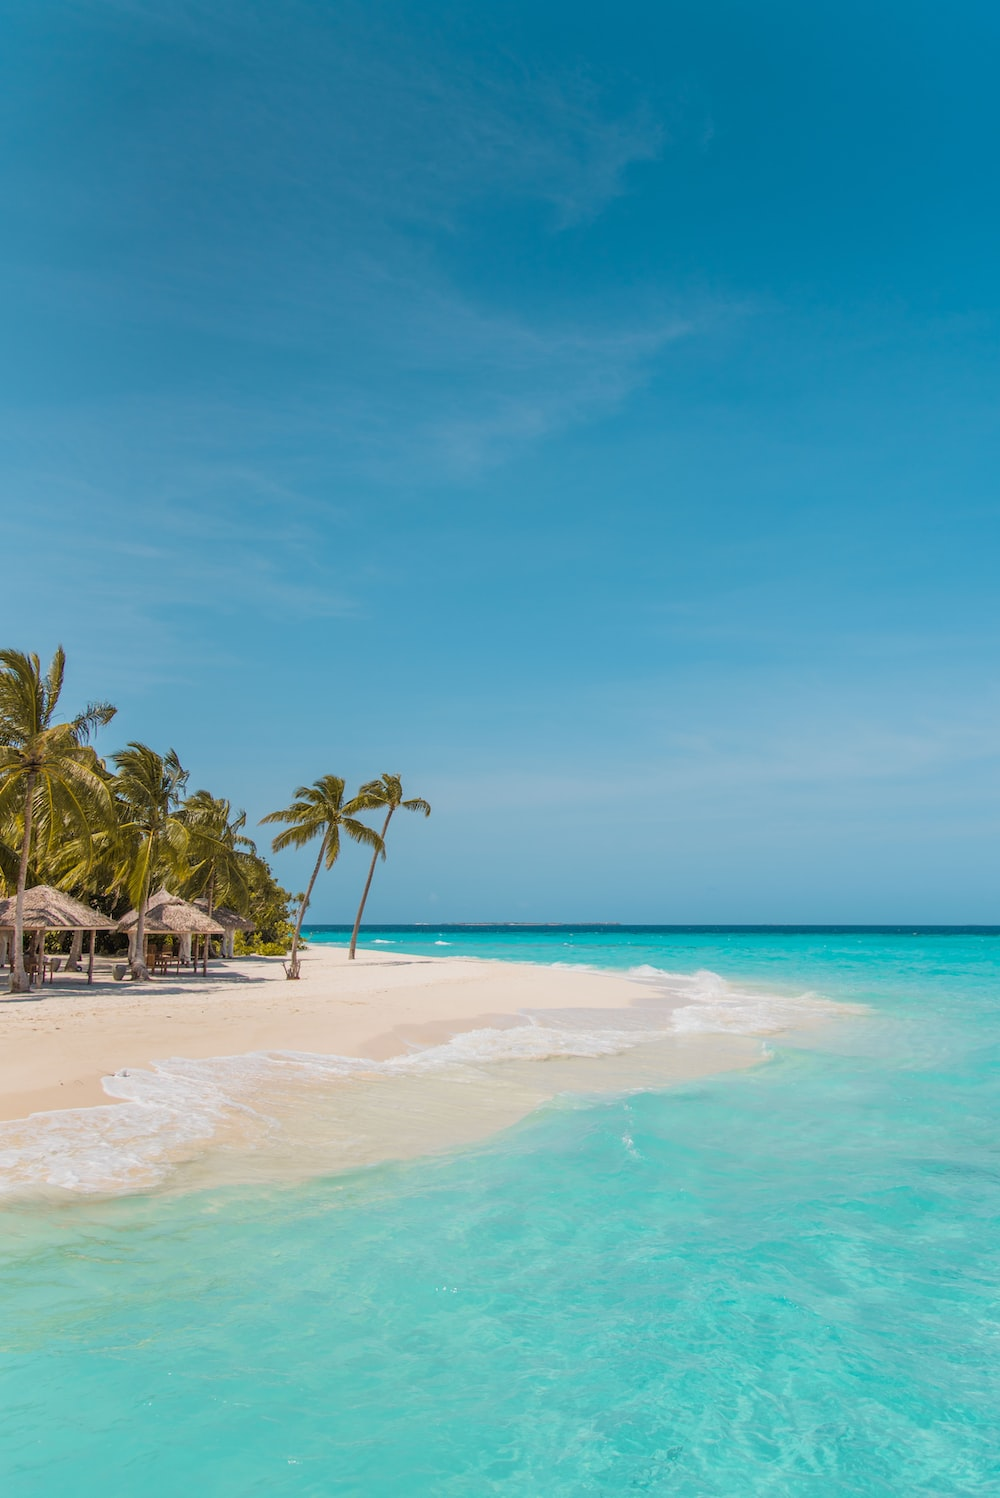
\includegraphics[width=\paperwidth,height=\paperheight]{Beach.jpg}
  }%
}
\usepackage{graphicx}
\graphicspath{ {./images/} }

\usepackage[pagestyles]{titlesec}
\titleformat{\chapter}[display]   
{\normalfont\huge\bfseries}{\chaptertitlename\ \thechapter}{20pt}{\Huge}   
\titlespacing*{\chapter}{0pt}{-50pt}{40pt}
\titleformat{\chapter}[display]{\normalfont\bfseries}{}{0pt}{\Huge}
\newpagestyle{mystyle}
{\sethead[\thepage][][\chaptertitle]{}{}{\thepage}}
\pagestyle{plain}

\begin{document}


\begin{tikzpicture}[font=\sffamily,remember picture,overlay]
    \path (current page.north west) node[below right,fill={rgb:white,0.55;green,2.5;pink,1.5},minimum 
    width=\paperwidth,minimum height=3cm](box){};
    
    \path (box.west) node[right=7cm,align=center] %<distance can be changed to suit
    {{\fontsize{45pt}{65pt}\color{white}\textbf{Summary Examples}}\\[2mm]
    {\fontsize{30pt}{20pt}\color{white}Grass}\\[2mm]
    {\fontsize{10pt}{10pt}\color{white}August 2022}};
    
\end{tikzpicture}

\vspace{15mm}

\begingroup
\let\clearpage\relax
\tableofcontents

\mainmatter
\endgroup
\newpage

\chapter{Weather and Climate}
\begin{minipage}{0.5\textwidth}
\begin{enumerate}
  \item Latitude: Singapore is located 1 degree and 22 minutes north of the equator hence it has a tropical climate

  \item Altitude: Every 1000m increase in height leads to a decrease in 6.5 degrees celcius
  
  \item Distance from the sea: Anchorage and Fairbanks located in alaska at coastal areas and inland areas respectively have different mean monthly temperature. Anchorage has temperature range of -10 to 15 while fairbanks has temperature range of -25 to 16
  
  \item Cloud cover: Sahara desert that has little cloud cover has mean daily temperature of 10 to 40 while Singapore which has a lot of cloud cover has mean daily temperature of 23 to 31
  
  \item Variation in solar output: In 2000, number of sunspots recorded the highest in a few years at 165 observed
  
  \item Volcanic eruptions: Eruption of Mt Pinatubo in 1991 released 17 million tonnes of sulfur dioxide that lowered temperature for as much as 0.6 degrees celcius
  
  \item Deforestation: Between 2010 and 2015, 52000 square kilometres of rainforest was lost every year
  
  \item Agriculture: In Argentina, research shows that methane from cows accounts for as much as 30\% of the countries greenhouse emissions
  
  \item Industries: Manufacturing a mobile phone is equivalent to 60kg of CO2 while manufacturing a computer and a monitor is equivalent to 275kg of CO2. This is equivalent to a car travelling 38 times the length of the Pan Island Expressway in Singapore
\end{enumerate}
\vspace{1.5cm}
\end{minipage}
\begin{minipage}{0.5\textwidth}
  \begin{enumerate}
    \setcounter{enumi}{9}
    \item Sea level rise: Majuro Atoll in the Pacific Ocean will lose 80\% of its land if sea level rises by 0.5m
  
    \item More frequent extreme weather events: In August 2003, Europe experienced a heat wave that killed more than 70,000 people
    
    \item Spread of some infectious insect bourne diseases: In 2004, Nepal and Bhutan, countries which have cool temperate climates, experienced its first cases of dengue due to rise in temperatures
    \item Lengthening the growing season in certain regions: An increase in the type of crops can now be grown in UK. New crops such as blackberries and maize can now be cultivated
  
    \item International agreements: In 1997, the Kyoto protocol was first drawn up and came into force in 2005. Coutries like Finland, Iceland, Austria and Spain were set to reduce their greenhouse emissions by 5\% below their 1990 levels from 2008 to 2012
    
    \item National responses: \begin{itemize}
      \item Singapore Green Plan 2012, launched by Ministy of the Environment in 2002. This plan aimed to produce 60\% of Singapore’s energy needs using natural gas by 2012
      \item Green Mark Scheme lauched by Building Construction Authority in 2005. This scheme aims to encourge more new ‘green’ buildings, which are more energy efficient. ‘Green’ buildings like National Library building have reported energy savings of 15\% to 35\% compared to normal buildings
      \item Plant-A-Tree programme started in 1971 aims to maintain Singapore’s status as a Garden City by planting trees. The programme has planted an estimated 60,000 trees yearly
    \end{itemize} 
  \end{enumerate}
\end{minipage}

\newpage 
\chapter{Tourism}
\begin{minipage}{0.5\textwidth}
  \begin{enumerate}
    \item Scenic beauty: Victoria falls between the border of Zambia and Zimbabwe attracts around 300,000 visitors annually

    \item MICE: Singapore is a major MICE destination and has held many important events such as the World Bank Group in 2006 and Youth Olympic Games in 2010
    
    \item Medical facilities: South Korea is a popular destination for those seeking cosmetic surgery due to its advanced technology and skilled doctors
    
    \item Heritage tourism: Sites like Tower of London and Buckingham Palace atracts around 15 million people to london every year
    
    \item Film-induced tourism: Zhangjiajie National Forest Park in China gained many international tourist after being featured in the film Avatar. The park even renamed one of its rock columns as Avatar Hallelujah Mountain
    
    \item Pilgirmage tourism: The annual Hajj to Mecca, Saudi Arabia attracts around 1.8 million international tourists
    
    \item Dark tourism: Nanjing Massacre Memorial Hall was bulit to commemorate the murder and rape in Nanjing after the city was captured by Japanese in December 1937
    
    \item Government: STB promotes tourism in Singapore and encourages tourism-related businesses to invest in Singapore. Such as hotels, resorts, cruises and airlines
    
    \item Media: Media influence has resulted in places like Antartica, Himalayas mountain and long-distance cruises to become more popular forms of tourism
    
    \item International Organisation: OECD tourism committee meets regularly to promote sustaniable tourism. The address economic, sustainability and employment issues related to tourism
  \end{enumerate}
  \vspace{0.1cm}
\end{minipage}
\begin{minipage}{0.5\textwidth}
  \begin{enumerate}
    \setcounter{enumi}{10}
    \item Better and affordable transport: Airbus A380 is a plane that can carry about 853 passengers and can fly at a speed of 1050km/h. It takes around 14 hours for a flight from Singapore to London in the plane
    
    \item Disposable income: China and India has experienced economic growth and this has allowed more people to be in the middle and high income groups due to higher disposable income
    
    \item Leisure time: In Australia, employees can exhcange paid overtime work for leave. This allows more employees to have longer weekend breaks
    
    \item Attractions: Dubai is a major tourist destination due to its tourist attraction such as the Palm Islands and Burj Al Arab
    
    \item Investment in infrastructure and services: In 2012, Changi airport’s budget terminal was closed down to make way for the new terminal 4 which was completed in 2017
    
    \item Disasters: By the end of 2011, Japans international tourist arrivals was down by 28\% to 6.2 million people due to the Tohuku earthquake in March 2011
    
    \item Recessions: The Global Financial Crisis which occured in 2007 and 2008 caused economies to slow down and resulted in less people travelling overseas for tourism
    
    \item Political situations: During the civil war in 2011 in Libya, many governments banned flights to Libya. By the end of 2011, Libya there was no commercial airlines landing in Libya and no tourist arrivals
    
    \item Diseases: During the SARS outbreak in 2003, Singapore’s international tourist arrivals was down by 67\% and Singapore was on WHO’s list for SARS infected countries
    
    \item Employment opportunities: In 2011, UNWTO estimated that tourism employs about 235 million people worldwide
  \end{enumerate}
\end{minipage}

\newpage
\begin{minipage}{0.5\textwidth}
  \begin{enumerate}
    \setcounter{enumi}{20}
    \item Growth in income: Fishermen are payed a significant amount of US\$80 to US\$100 per boat for their services in Philippines
    
    \item Development in infrastructure: Both Athens, Greece and Beijing, China, expanded their underground railways networks in the 2004 and 2008 Summer Olymic Games respectively
    
    \item Seasonal employment: In places like skii resorts, there is high employment rates during the winter but low employment rates in the summer
    
    \item Under-use of facilities: Parts of the Beijing National Aquatics Centre, built for the 2008 Summer Olympic Games, was renovated in 2010 to be a water park
    
    \item Preservation of local customs and heritage: Entry fees to areas like the Great Pyramid of Giza is used to help fund conservation efforts
    
    \item Dilution of local customs and heritage: Due to the hefty fees to enter the village of the Kayan Lahwi women, many tourists act like the women are artefacts and constantly pictures
    
    \item Conservation of natural environments: In Kenya, the money raised from wildlife tourism is used to preserve animals and their habitats
    
    \item Vandalism: The stones and bricks on the Great Wall of China, which attracts around 10 million people annually, is covered in graffiti
    
    \item Littering and pollution: Soild and liquid waste are dumped into the Caribbean Sea by ships due to limited land space
    
    \item Destruction of habitats: Egypt’s Red Sea is a popular tourist destination for diving. However the constant picking of rocks and coral by divers has damaged the coral reefs
    
    \item Carbon footprint: The carbon footprint of a flight from Singapore to Kuala Lumpur is 10kg of carbon dioxide per person
  \end{enumerate}
\end{minipage}
\begin{minipage}{0.5\textwidth}
  \begin{enumerate}
    \setcounter{enumi}{31}
    \item Conservation of fragile environments: Due to its diverse ecosystem and beauty and to ensure that it is preserved, Australia’s Great Barrier Reef earned its place on the UNESCO World Hertiage Site list in 1981
    
    \item Tensions between tourists and locals: In 2012, Indonesia’s Central Statistics Agency recorded 2.9 million international tourists. This large amount of tourists created some tensions between tourists and locals such as opinions between public displays of affection
    
    \item Tensions between tourist and environment: Machu Picchu, Peru where local authorities banned the use of helicopters in fear of noise disturbance to indigenous wildlife. The heavy footsteps of tourists visting Machu Picchu every year also slowly damages the land and artefacts
    
    \item Local communities: Village of Candirejo in Central Java, Indonesia, set up a cooperative in 2003 to manage and implement their own tourist-related programmes. By 2004, the village had 22 homestays, 22 local horse-drawn carts and 6 local restaurants
    
    \item Visitors: In 2007, the Tourism Sustainability Group encouraged tourists to select their holiday destination based on the conservation efforts of the place to minimise their carbon footprint
    
    \item Tour operators: Phuket Alternative Tours set up in 2006 by tour operators ensures that their tours are sustainable and that people who sign up participate in ecotourism
    
    \item Planning authorities: STB has implemented programmes to ensure ethnic districts are conserved in Singapore. Such districts include Chinatown, Little India and Kampung Glam
    
    \item NGOs: Since 1990s, the international Ecotourism Society has developed guidlines, conducted training courses and published research papers related to tourism and the environment to promote ecotourism
  \end{enumerate}
  \vspace{0.4cm}
\end{minipage}

\newpage
\chapter{Plate Techtonics} \small
\begin{minipage}{0.5\textwidth}
  \begin{enumerate}
    \item Destruction by volcanic materials: The eruption of Kilauea in Hawaii in 1983 destroyed many houses and highways

    \item Landslides and Lahars: The eruption of Mt Merapi in 2010 trigerred landslides and lahars that killed over 300 people
    
    \item Pollution: The eruption of Mt Pinatubo in 1991 resulted in major air pollution that affected many people
    
    \item Effects on weather: Eruption of Mt Tambora in 1815 caused global temperatures to drop by 1.7 degrees
    
    \item Fertile soil: The volcanic soils of Java and Bali support the cultivation of coffee, tea and rice
    
    \item Precious stones, minerals and building materials: In East Java and Bali, workers collect sulfur from active volcanoes
    
    \item Tourism: The Roman town of Pompeii wich was buried by lava and ashes when nearby Mt Vesivius erupted in 79CE is now attracts over 3 million tourists every year
    
    \item Geothermal energy: Most of Iceland’s electricity is generated by geothermal energy and 70\% of homes in Iceland is heated by volcanic steam
    
    \item Population density: Christchurch New Zealand, February 2011, magnitude 6.3, 180 deaths
    
    \item Level of prepardness: Tohuku Japan, March 2011, magnitude 9.0, 28,000 deaths
    
    \item Time of occurance: Sun-moon lake Taiwan, 1999, magnitude 7.6 2,400 deaths. Earthquake occured after midnight

    \item Distance from epicentre: Haiti, January 2010, magnitude 7.0, 223000 deaths. Earthquake occured in capital city
    
    \item Soil type: Christchurch New Zealand, February 2011, magnitude 6.3, 180 deaths
    
    \item Fire: Kobe Japan, January 1985, magnitude 7.2, 6,500 deaths

    \item Landslides: Sichuan China, May 2008, magnitude 7.9, 100,100 deaths
    
    \item Loss of lives: Tohuku japan, March 2011, magnitude 9.0, 2,800 deaths
    
    \item Destruction of properties: Kobe Japan, January 1985, magnitude 7.2, 6,500 deaths
  \end{enumerate}  
\end{minipage}
\begin{minipage}{0.5\textwidth}
  \begin{enumerate}
    \setcounter{enumi}{17}
    \item Destruction of infrastructure: Aceh Indonesia, December 2004, magnitude 9.2, 228,000 deaths
    
    \item Destruction of services: Sichuan China, May 2008, magnitude 7.9, 100,100 deaths
    
    \item Rescue and recovery: After the 2011 earthquake in Tohuku Japan, there was only a limited time of 3 days for search and rescue
    
    \item Providing immediate healthcare, food and water: After the 2010 earthquake in Haiti, looting and fighting broke out due to a shortage of food supplies
    
    \item Rebuilding of stronger infrastructure: After the 1985 earthquake in Kobe Japan, Japan spent billions developing technology for earthquake resistant buildings
    
    \item Provision of healthcare: After the 2011 earthquake in Christchurch New Zealand, there were more reported cases of people having health issues such as anxiety and depression. Resulting in more health workers being deployed.
    
    \item Land use regulations: In California, USA, all new buildings development are not built across fault lines or low lying areas where risks of liquefaction is high
    
    \item Infrastructure: The Taipei 101 is reinforced using heavy steel bars and reinforced concrete. On top of that, it is also fitted with a dampening device that absorbs seismic energy
    
    \item Emergency drills. Since 1960, Japan conducts and annual emergency drill on 1st September to commemorate Disaster Prevention Day
    
    \item Earthquake monitoring devices: In Japan, earthquake monitoring sensors are fitted on roads and bridges to help detect potential earthquakes
    
    \item Tsunami monitoring and warning systems: Deep sea tsunami detectors are located in Hawaii, USA to monitor and predict paths of tsunamis
  \end{enumerate}  
  \vspace{2.7cm}
\end{minipage}

\newpage
\normalsize
\chapter{Food Resources} \small
\begin{minipage}{0.5\textwidth} 
  \begin{enumerate}
    \item Disposable income: From the 1950s to 1990s, taiwan experienced a surge in economic growth which led to the population demanding 4 times as much meat

    \item Pricing: From 2006 to 2009, the global food crisis pushed over 100 million people worldwide into chronic food hunger and starvation
    
    \item Food preference: Growth in India’s economy resulted in Indian’s life becoming more hectic. This resulted in India spending \$400 million on fast food in 2009
    
    \item Organic food: A research done in 2011 in the USA showed that about 58\% of the population in the USA preferred organic food to inorganic food
    
    \item Population growth: By 2025, the population in the Sub-Saharan Africa is expected to be so large that it must completely rely on food aid for food
    
    \item Stability of food: Singapore imports 90\% of its food hence it is important to have high food security in Singapore
    
    \item Civil war: In April 2011, food stock in Libya dropped rapidly due to a civil war
    
    \item Natural disaster: In 2008, a severe drought in Zimbabwe caused major food shortage
    
    \item Malnutrition: WHO estimated that 250000 to 300000 Vitamin A deficiency children go blind every year
    
    \item Starvation: In Mali 2012, 5 million people faced hunger and starvation due to a poor harvest that led to a civil war
    
    \item Lower productivity: In coutries like India and Ethiopia, lower level of nutrition intake resulted in lower productivity
    
    \item Long term debt: A research done in 2005, 2006 and 2009, food provided as aid is up by 34\% more compared to food purchased locally
    
    \item Social unrest: In Mozambique 2010, food prices increased due to a drought that resulted in wheat prices increasing by 30\%. This led to a violent protest that killed and injured many people
    
    \item Obesity: From 1971 to 2000, obesity rates in USA increased from 15\% to 31\%
  \end{enumerate}
\end{minipage}
\begin{minipage}{0.5\textwidth}
  \begin{enumerate}
    \setcounter{enumi}{14}
    \item Lower productivity: A research done in Duke University showed that employees with BMI of higher than 40 were twice as likely to fall sick. Resulting in higher compensation claims by the University
    
    \item Food wastage: Food wastage in DCs ranges from 95 to 115 kg per capita. This is significantly higher as compared to LDCs where food wastage eanges from 6 to 11kg per capita
    
    \item Dieting: In 2012, the weight loss industry in USA was estimated to be worth \$200 billion
    
    \item Climate: Crops like strawberries and coffee grow best in cool temperate climates while crops like rice grow best in warmer climates
    
    \item Relief: Crops like coffee, tea and strawberries grow best in higher relief where there are cooler temperatures
    
    \item Soil and draniage: Crops like rice require a lot of water hence they are grown on soil that can retain water such as clay
    
    \item Government policies: In India 2012, the Punjab Departement of Agriculture helped up farmers by providing education on best variety of seeds, pesticides treatement and irrigation methods to increase crop production in India
    
    \item Technology: From the 1960s to 1990s, India was intoduced to a high yielding variety of rice seeds which pulled the country out of famine and starvation
    
    \item Purpose of farming: In less developed countries like Africa, people usually practise subsistance farming which is very labour intensive and have very low capital while in developed countries like USA, people usually practise commercial farming which heavily relys on technology and big areas of land. Crops are usually exported
    
    \item Demand and capital: China used to be a producer and exporter of corn but as the economy grew, people started demanding meat products
    
    \item Salinisation: In Murray-Darling bay in Victora Australia, due to its low lying terrain and high evaporation rate, followed by human activities such as land clearing and irrigation, the area experienced salinsation and the land is unsuitable to cultivate crops
  \end{enumerate}
\end{minipage}

\newpage
\begin{enumerate}
  \setcounter{enumi}{25}
  \item Eutropication: In USA, it was discovered that pesticides and fertilisers from farms contaminated groundwater. Since 23\% of freshwater used in the USA comes from groundwater. This is a major problem
    
    \item Climate change: If temperature continues to increase, countries like Brazil, India, Pakistand and certain parts of the USA is expected to have a decrease of 50\% of food production over time
    
    \item Extreme weather events: In 2006, cyclone Larry caused Queensland to experience food shortage as crops like Mangoes, bananas and strawberries were destroyed
    
    \item Pests: In 2009, Liberia in Northern parts of Africa was declared a state of emergency after tens of million caterpillars invaded and destroyed crops and plants in their way
    
    \item Civil strife: In May 2012, the syrian village of Houla experience food shortage after a civil strife that killed 100 people
    
    \item Poor governance: In India, the state of Madhya Pradesh in 2010, 40000 people faced food shortage due to diversion of land and financial resources to developing a mine, steel plant and port
    
    \item Rising demand of meat: Brazil, Russia, India and China are LDCs that have great economies that contribute to the world’s economy. Because of this, wealthy people in these countries demand a lot of meat
    
    \item Soaring cost of fertiliers: In March 2011, world crude oil prices increased by 10.3\%. This resulted in Kazakhstan, a major producer of wheat to increase its price of exported wheat
    
    \item Biofuel crops: A reasearch done by US department of agriculture in 2009 showed that 25\% of crops grown in the USA is used as biofuel. This is equivalent to to food that can feed 330 million people for a year
\end{enumerate}

\vspace*{\fill}
\begingroup
\let\clearpage\relax
\chapter{References}
\endgroup
Complied from: \href{https://www.reddit.com/r/SGExams/comments/iuka5m/o_levels_e_geog_compilation_of_all_examples/}{[O Levels] E Geog Compilation of all Examples}:\\ \footnotesize
\begin{enumerate}
  \item \href{https://www.reddit.com/r/SGExams/comments/9sm2o5/o_level_e_geog_weather_climate_case_studies/?utm_source=share&utm_medium=ios_app&utm_name=iossmf}{[O Level] E Geog Weather \& Climate Case Studies}
  \item \href{https://www.reddit.com/r/SGExams/comments/9sm2tv/o_level_e_geog_tourism_case_studies/?utm_source=share&utm_medium=ios_app&utm_name=iossmf}{[O Level] E Geog Tourism Case Studies
  } 
  \item \href{https://www.reddit.com/r/SGExams/comments/9sm2iq/o_level_e_geog_plate_techtonics_case_studies/?utm_source=share&utm_medium=ios_app&utm_name=iossmf}{[O Level] E Geog Plate Techtonics Case Studies
  }
  \item \href{https://www.reddit.com/r/SGExams/comments/9sm30b/o_level_e_geog_food_resources_case_studies/?utm_source=share&utm_medium=ios_app&utm_name=iossmf}{[O Level] E Geog Food Resources Case Studies
  }
\end{enumerate}

\end{document}